\newpage
\section{Implementierung}

Wie in Kapitel \ref{sec:Architektur} bereits erwähnt ist die Applikation dem Design-Pattern Model-View-Controller nachempfunden. Im Folgenden wird die konkrete Implementierung beschrieben und die Architektur mittels Codebeispielen konkretisiert.
\\
Der allgemeine Ablauf der Anwendung sieht lediglich einen Aufruf der HTML-Seite index.html vor. In diese wird mittels Javascript der jeweilige Inhalt (eine View) geladen und mit Daten und Funktionen (über den Controller) versorgt.
\begin{figure}[h]
\centering
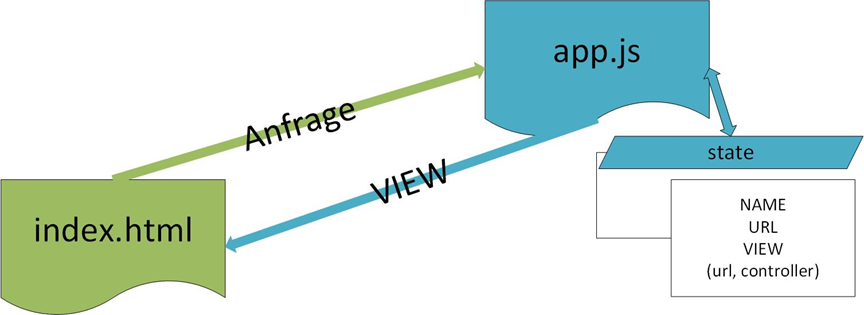
\includegraphics[width=1\textwidth]{ref/images/index.png}
\caption[Ablauf Applikationsdarstellung]{Ablauf Applikationsdarstellung}
\label{fig:HTML-Darstellung}
\end{figure}

App.js ist eine Javascript-Datei, die unter Anderem die Zuordnung der Views zu ihrem jeweiligen Controller durchführt. 
\subsection[App.js]{App.js
 \\ \textnormal{\small{\textit {Verfasst von Melanie Hammerschmidt}}}}
 
In der app.js ist pro View ein Status (state) hinterlegt, der alle folgenden Informationen definiert:
\begin{itemize}
\item Name des Status
\item URL (innerhalb der App)
\item View-Bezeichnung (URL der View/Vorlage, Controllername)
\end{itemize}

\newpage
Konfiguriert wird ein solcher Status beispielsweise wie folgt:
\begin{lstlisting}
.state('tab.play', {
    url: '/play',
    views: {
      'tab-play': {
        templateUrl: 'templates/tab-play.html',
        controller: 'PlayCtrl'
      }
    }
  })
\end{lstlisting}

Die Informationen über die aktuell gewählte View gibt app.js an index.html zurück, welche sie nach außen dem Nutzer darstellt.


App.js wird bei jedem Start der Applikation zuerst geladen. Dabei findet auch immer eine Prüfung der aktuellen Internetverbindung statt. Internet wird für die Darstellung des Kartenmaterials benötigt. Die Konsequenz einer fehlenden Internetverbindung ist demnach ein Abbruch der Applikation.

Standardmäßig wird bei korrektem Startverhalten die play-View in die index.html geladen. Das ist eine ebenfalls in app.js definierte Defaulteinstellung. Die folgende Codezeile wird demnach dann aufgerufen, wenn der URL-Provider keine zu einem Status passende URL finden kann. In diesem Fall wird die URL auf die des tab.play-Status gesetzt.
\begin{lstlisting}
  $urlRouterProvider.otherwise('/tab/play');
\end{lstlisting}

\subsection[Controller und Services]{Controller und Services
 \\ \textnormal{\small{\textit {Verfasst von Melanie Hammerschmidt}}}}

Für jede View existiert ein Controller, der dann die alleinige Macht über Model-Aufrufe für die View hat. Der Begriff Model wird im Folgenden durch den Cordova-spezifischen Begriff Service ersetzt. Alle folgenden Statusbeschreibungen trennen View, Controller und Model bildlich voneinander. Insgesamt wurden für die Applikation drei Services entwickelt:
\begin{itemize}
\item \emph{Player Service}: Zuständig für die Behandlung von Spielerdaten
\item \emph{Location Service}: Zuständig für Positionierungsaufgaben und die Handhabung der Lokalisierung
\item \emph{Task Service}: Zuständig für Aufgabenerstellung und -management
\end{itemize}
\subsection[Applikationsaufbau]{Applikationsaufbau
 \\ \textnormal{\small{\textit {Verfasst von Melanie Hammerschmidt}}}}
 
Die App besitzt einen getabbten Aufbau. Das heißt es existiert eine Kopfzeile, die dem Nutzer vier verschiedene Tabs anbietet: Spielen, Highscores, Account und Credits. 
\\
Die angezeigten Tabs der Applikation sind ein Spezialstatus, der in app.js als abstrakt gekennzeichnet ist und ständig im Hintergrund aktiv ist. Die Tabs sind auch wieder als HTML-Template definiert.
\begin{lstlisting}
.state('tab', {
    url: "/tab",
    abstract: true,
    templateUrl: "templates/tabs.html"
  })
\end{lstlisting}
Alle folgenden Tabs bauen auf diesem abstrakten Status auf.
\begin{figure}[h]
\centering
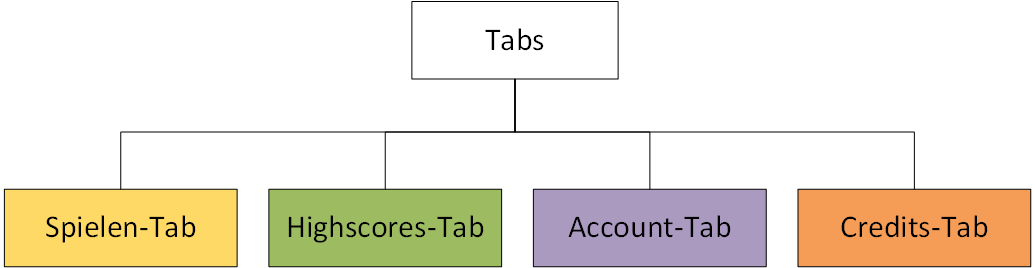
\includegraphics[width=1\textwidth]{ref/images/tabs.png}
\caption[Tabaufbau]{Tabaufbau}
\label{fig:Tabaufbau}
\end{figure}

Jeder der Tabs wird im Folgenden näher beschrieben werden.
\newpage
\subsubsection[Spielen-Tab]{Spielen-Tab
 \\ \textnormal{\small{\textit {Verfasst von Melanie Hammerschmidt}}}}
 
Der Spielen-Tab bietet dem Nutzer die Möglichkeit ein Spiel zu starten. Er gibt dafür einen Namen und einen Spielradius an. Unter dieser Kombination wird er später seinen Highscore dieses Spiels finden können. 
\\
Die View, die dahinter steht ist anfangs die Play-View, welche prinzipiell im Spielen-Tab als Startseite der Applikation angezeigt wird. Im Verlauf des Spiels wird der Nutzer auf verschiedene View weitergeleitet, die im Folgenden näher beschrieben werden. 
\begin{figure}[h]
\centering
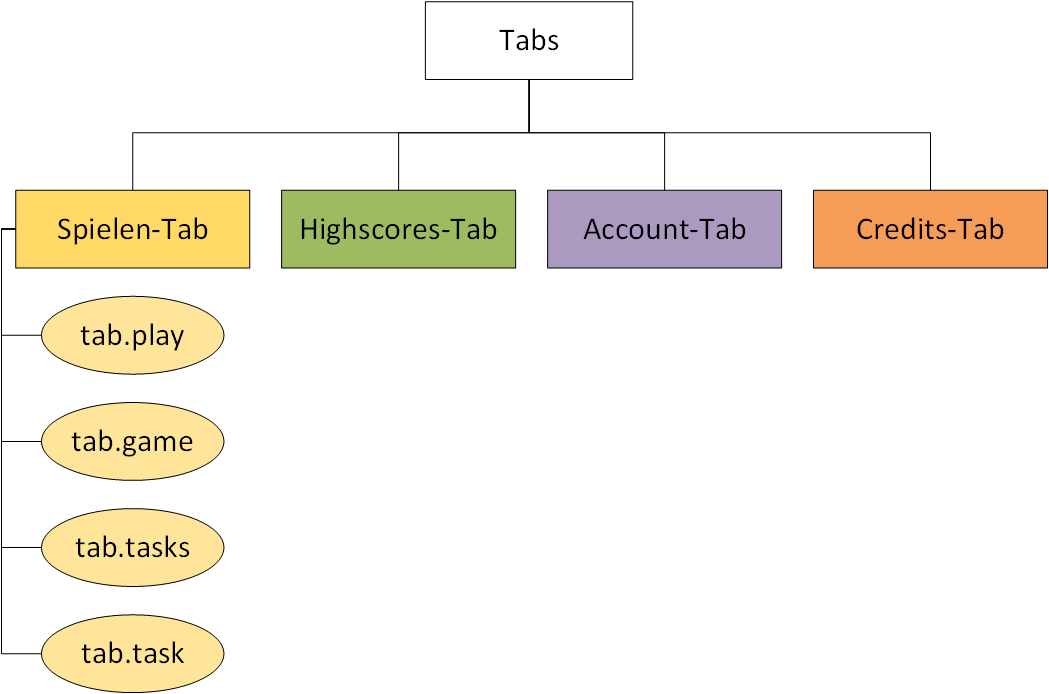
\includegraphics[width=1\textwidth]{ref/images/tabs_spielen.png}
\caption[Tabaufbau Spielen-Tab]{Tabaufbau Spielen-Tab}
\label{fig:Tabaufbau Spielen-Tab}
\end{figure}

\newpage
\paragraph{Play-View}
%
%Beschreibung der HTML-Seite
Die Play-View hat ein Textfeld, dass den Spielernamen übernehmen kann und eine Selectbox, die den Radius auf zwei bis fünf Kilometern beschränkt. Bei fehlender Eingabe wird auf drei Kilometer als Defaultwert gesetzt. Außerdem bietet die View einen Button, der das Spiel startet. 
%
%Ablaufplan
\begin{figure}[h]
\centering
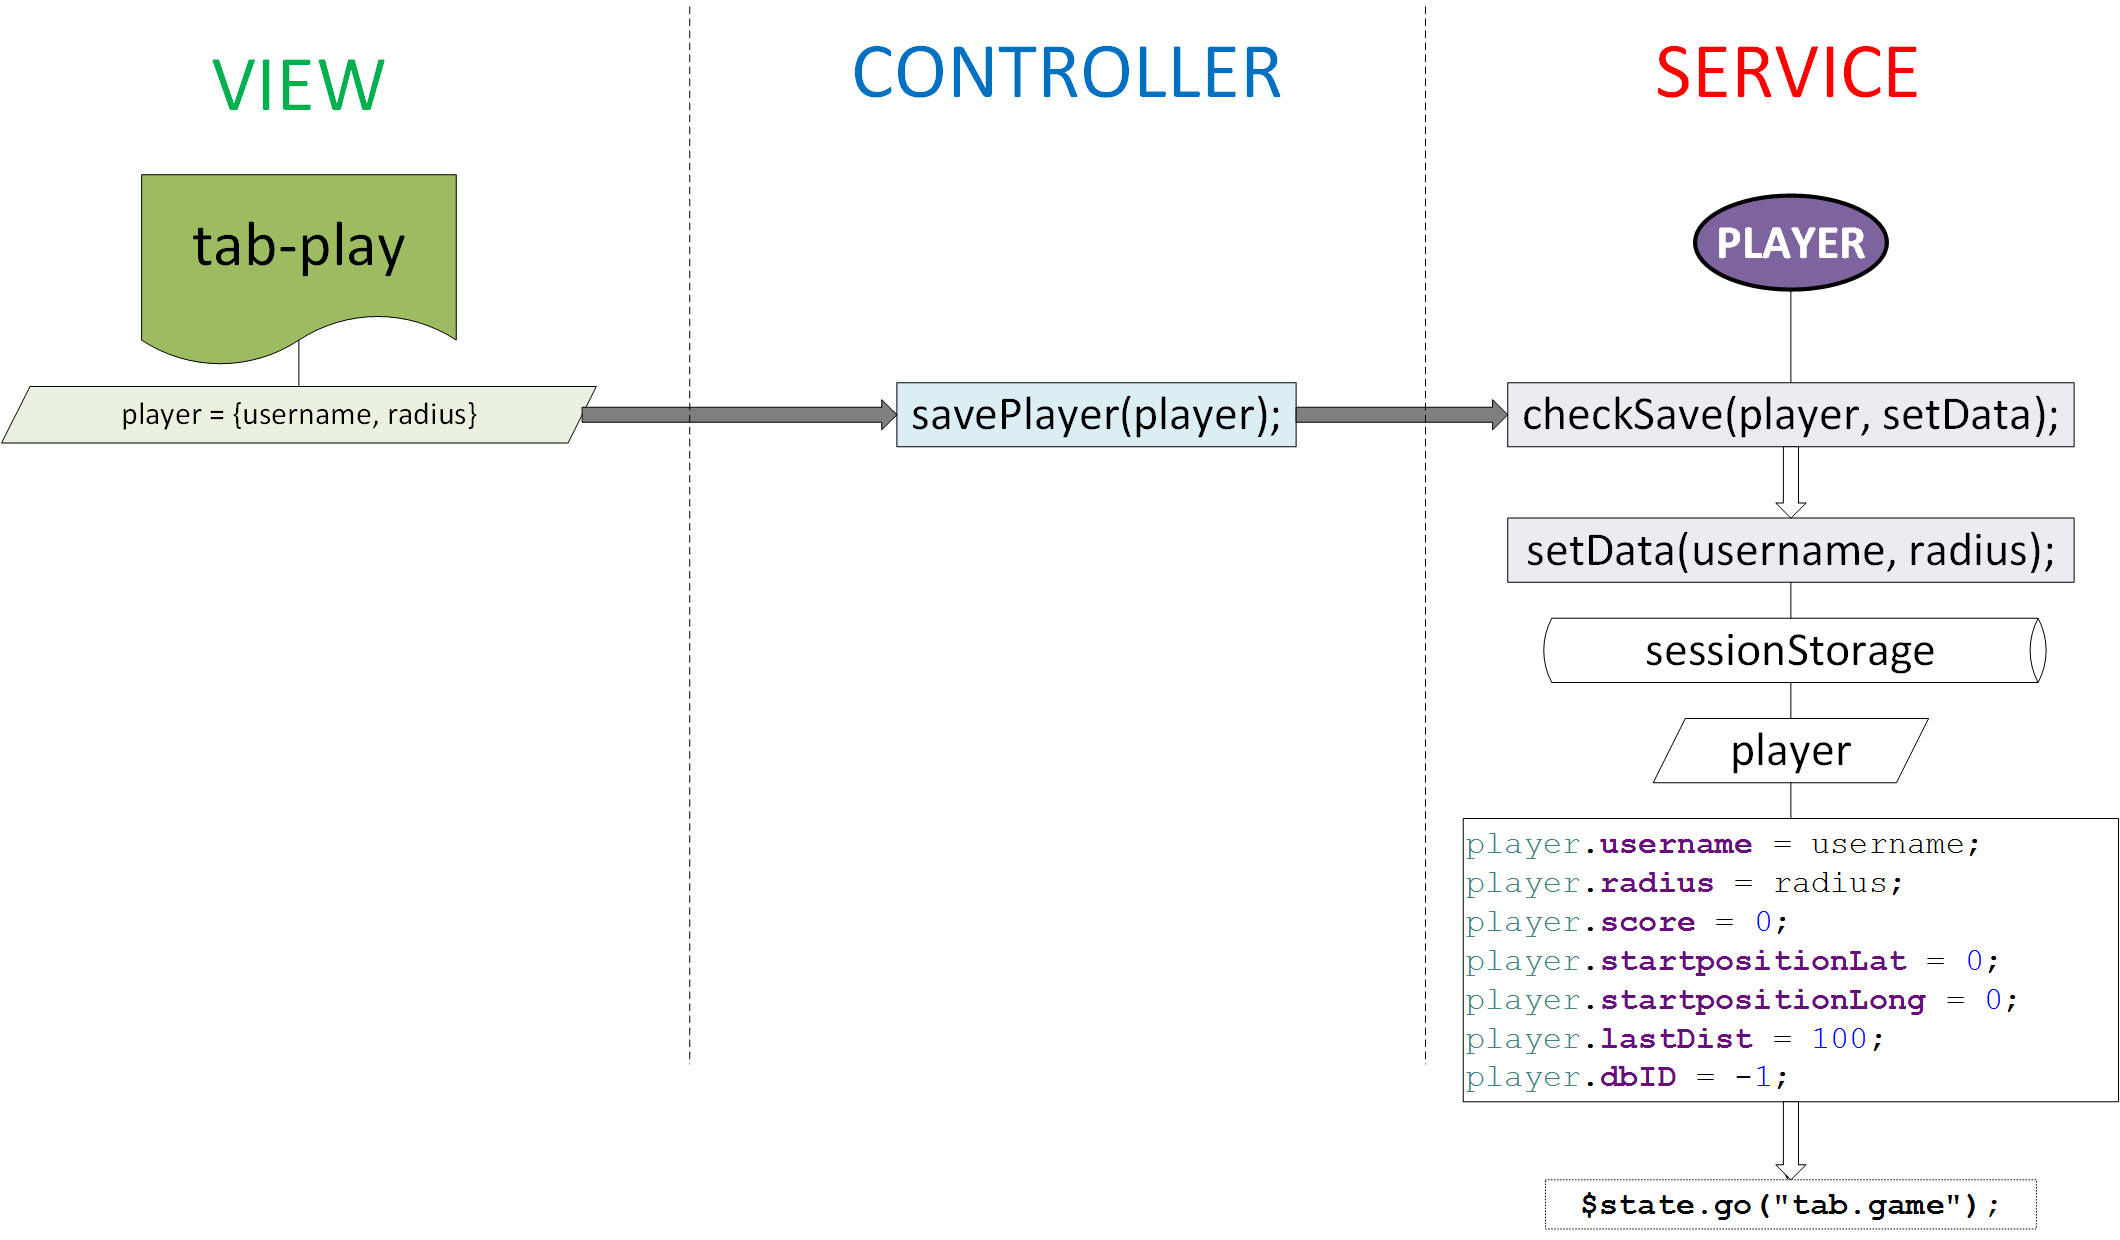
\includegraphics[width=0.8\textwidth]{ref/images/02-play-tab.png}
\caption[Model-View-Controller: Play-View]{Model-View-Controller: Play-View}
\label{fig:MVC:Play-View}
\end{figure}
\\
%
% Beschreibung des Controllers und der Services
Der Play-View wurde über app.js der Controller 'PlayCtrl' zugewiesen, der wiederum Zugang zum Service 'Player' besitzt. Der \emph{Player Service} kapselt alle Funktionen, die mit den Nutzerdaten im Zusammenhang stehen.
\\
% Verwendungszweck
Schon während der Eingabe der benötigten Informationen (Name und Radius) wird ein Javascript-Objekt 'player' generiert, das diese Daten enthält. Mit Druck auf den Button 'Los gehts' wird dieses Objekt an die Funktion 'savePlayer' des Controllers übergeben. 
\\
Der Controller leitet bei Aufruf dieser Funktion die Objektdaten Name und Radius an den dazugehörigen Service, der zuerst auf gültige Befüllung des Spielernamen prüft und bei Befüllung diesen speichert. Der dafür genutzte Speicher ist der sessionStorage des Geräts, der für die Dauer der Session die Daten des Spielers als Objekt mit den folgenden Eigenschaften speichert: 
\begin{enumerate}
\item Spielername und Radius: beides über Nutzer eingegeben und über Controller an Service zur Speicherung übergeben
\item Score: Punktestand des Spielers
\item StartpositionLat: Breitengrad der Startposition
\item startpositionLong: Längengrad der Startposition
\item lastDist: letzte Distanz zum Ziel für Verlaufsvergleich
\item dbID: ID des Spielers im Spielerarray des Sessionstorage
\item lastUpdate: Zeitpunkt der letzten Änderung
\end{enumerate}
Die noch nicht existierenden Werte werden mit Defaultwerten gefüllt.
\\
Wenn der Spielername nicht angegeben wurde erhält der Nutzer eine Aufforderung und das Spielerobjekt wird nicht weitergeleitet/gespeichert. Bei erfolgreichem Speichern hingegen erfolgt über den Service eine Weiterleitung in den Status 'tab-game' bzw. auf die Game-View.

\paragraph{Game-View}
%Beschreibung der HTML-Seite
Die Game-View liegt ebenfalls im Tab 'Spielen' und ist für die aktuelle Standortbestimmung - also die Bestimmung des Startpunkts des Nutzers zuständig.


Sie besitzt anfänglich lediglich einen Button, über den man die Positionsbestimmung anstoßen kann. Bei fehlerfreier Ermittlung wird dem Nutzer eine Open Street Map mit seiner Position und dem eingezeichneten Radius angezeigt, sodass er einen Überblick über sein 'Spielfeld' bekommt. Außerdem wird ein weiterleitender Button eingeblendet, über den der Spieler die Spielmöglichkeiten in seinem berechneten Umfeld angeboten erhält.
Bei Fehlern bei der Positionsbestimmung erhält der Nutzer anstelle der Karte und des Button schriftliche Rückmeldung über die Art seines Fehlers.
%
%Ablaufplan
%
\begin{figure}[h]
\centering
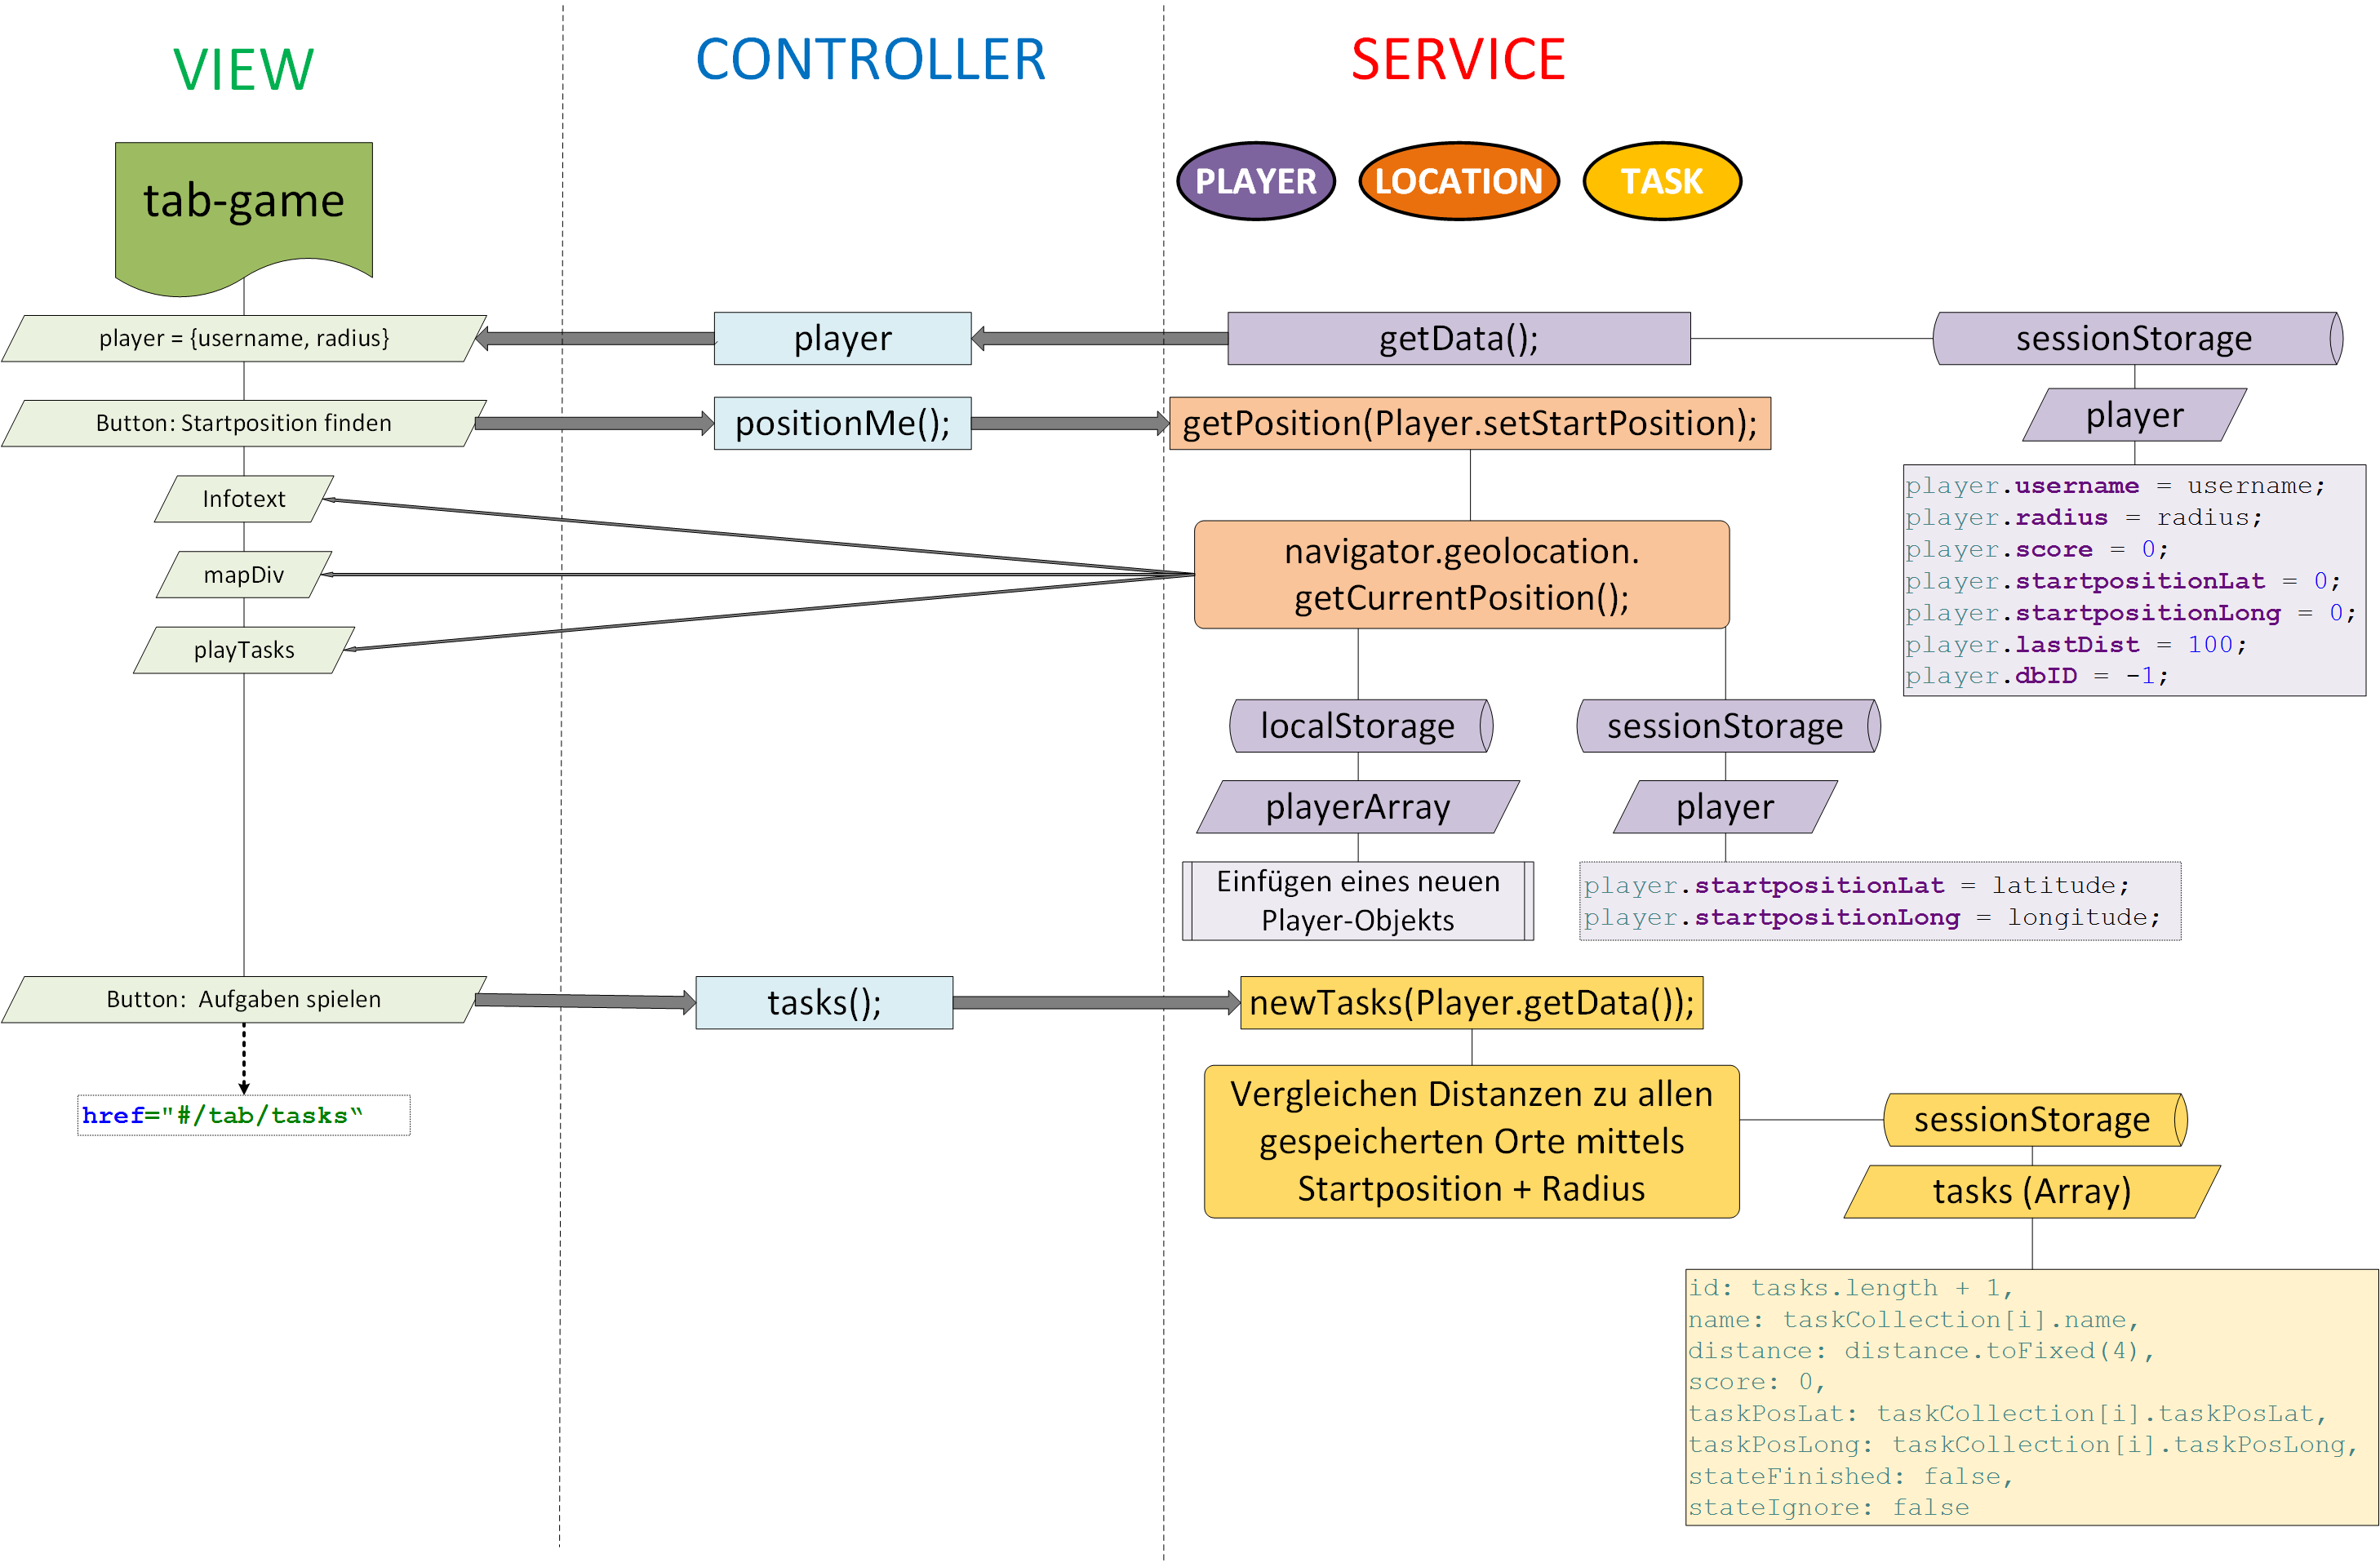
\includegraphics[width=0.8\textwidth]{ref/images/03-game-tab.png}
\caption[Model-View-Controller: Game-View]{Model-View-Controller: Game-View}
\label{fig:MVC:Game-View}
\end{figure}
%
% Beschreibung des Controllers und der Services
%


Die Game-View ist an den Controller 'GameCtrl' gebunden, welcher auf drei verschiedene Services zugreifen kann: \emph{Player}, \emph{Location} und \emph{Task}.

Der \emph{Player Service} kümmert sich, wie erwähnt um die Nutzerdaten. Der \emph{Location Service} wurde entwickelt, um die Positionsbestimmung und die Behandlung der Koodinatendaten zu kapseln. Der \emph{Task Service} hingegen gewährleistet die Generierung, Verfolgung und Speicherung der Aufgaben (Tasks) der ganzen Applikation.
\\
% Verwendungszweck
Die Nutzung der Applikation sieht eine Bestimmung der Startposition eines Spielers vor Erstellung der Aufgaben vor. Der Spieler erhält auf der Game-View eine kurze Übersicht seiner bisher gemachten Angaben (Spielername und Radius). Dieser werden vom Controller vor dem endgültigen Laden der View beim \emph{Player Service} angefragt (getData()). Der Service muss dafür auf den Sessionstorage des Geräts zugreifen und das 'player'-Objekt auslesen.


Nach dem Laden der View kann der Nutzer dann über den Button 'Startposition finden' seine aktuelle Position bestimmen lassen. Mit Klick auf den Button wird über den Controller, bzw. über seine Funktion 'positionMe', die Funktion des \emph{Location Service} aufgerufen werden ('getPosition'). Diese Funktion ist nicht nur für die eigenliche Bestimmung der Koordinaten, sondern auch für die Speicherung jener Daten verantwortlich.
%\\
%Dafür werden ihr die Spielerdaten über das Objekt 'player' übergeben und die Funktion zur Speicherung der Daten als Javascript-%Callback Funktion im Falle einer korrekten Ermittlung.
\\
\\
Der Befehl 'navigator.geolocation.getCurrentPosition()' ist der Weg, um auf die Geolokationsfunktionen von Cordova, bzw. des Geräts zuzugreifen. Nach diesem Aufruf werden die Felder der Game-View (Infotext, mapDiv und playTasks) entsprechend gefüllt und bei erfolgreicher Durchführung die Startpositionsdaten des Spielers %(vgl. Callbackfunktion) 
im Sessionstorage aktualisiert und der Spieler in das Spielerarray des Localstorage integriert. Der Localstorage des Geräts enthält im Vergleich zum Sessionstorage zu jeder Zeit seine Daten und wird nicht automatisch gelöscht. Das Array enthält also alle Spieler, die dann später auch im Highscore aufgelistet werden können.
\\
Wenn es bei der Positionierung zu Problemen kommt, erhält der Nutzer Rückmeldung nachdem die Timeout-Zeit von 30 Sekunden abgelaufen ist.
\\
Bei erfolgreicher Positionierung werden die Koordinaten über das mapDiv, einem Bereich der Game-View, in einer Open Street Map dargestellt (vgl. Kapitel \ref{sec:kartenmaterial}). Außerdem wird in diesem Fall der Button 'Aufgaben spielen' eingeblendet.
\\
Wird dieser Button daraufhin gedrückt, startet der Controller die Erstellung der Aufgaben für den Spieler.
\\
In dieser prototypischen Implementierung ist nur eine fixe Anzahl von Aufgaben implementiert, die von den Entwicklern frei bestimmt wurden und in einem Array gespeichert sind.
\\
Jede Aufgabe in dieser Sammlung hat folgende Informationen:
\begin{enumerate}
\item id: Identifikationsnummer der Aufgabe
\item name: schriftliche Bezeichnung der Aufgabe
\item taskPosLat: Aufgaben-Längengrad
\item taskPosLong: Aufgaben-Breitengrad
\end{enumerate}

Folgende Aufgaben sind im Prototypen implementiert. Es ist zu beachten, dass dies lediglich ein Auszug des Array ist, welches außerdem auch beliebig erweiterbar wäre.
\begin{lstlisting}
        var taskCollection = [
            {
                id: 0,
                name: "Mannheim Hbf",
                taskPosLat: 49.479904895467314,
                taskPosLong: 8.470357013095054
            },
            {
                id: 1,
                name: "Mannheim Universitaet",
                taskPosLat: 49.48373966279436,
                taskPosLong: 8.46222996711731
            },
            {
                id: 2,
                name: "Mannheim Wasserturm",
                taskPosLat: 49.48336089947494,
                taskPosLong: 8.477369150878872
            },
            {
                id: 3,
                name: "Mannheim Neckar",
                taskPosLat: 49.490776620594524,
                taskPosLong: 8.482561907531704
            },{
            ...
            }]
\end{lstlisting}

Der Controller ruft die Erstellung der Aufgaben für den Spieler über die Funktion 'newTasks' des \emph{Task Service} auf.
\\
Der Service berechnet daraufhin für jede Aufgabe in seiner Sammlung die Entfernung, die der Spieler zu der jeweiligen Position hätte und speichert sie in ein Spieler-Aufgabenarray, wenn die Distanz kleiner oder gleich dem vom Spieler gewählten Radius ist.
\\
Die Berechnung der Distanz erfolgt über die Funktion 'getDistance', welche im Folgenden aufgeführt ist.
\begin{lstlisting}
        function getDistance(lat1, lon1, lat2, lon2) {
            var R = 6371; // Radius der Erde in Kilometern
            var dLat = deg2rad(lat2 - lat1);
            var dLon = deg2rad(lon2 - lon1);
            var a =
                    Math.sin(dLat / 2) * Math.sin(dLat / 2) +
                    Math.cos(deg2rad(lat1)) * Math.cos(deg2rad(lat2)) *
                    Math.sin(dLon / 2) * Math.sin(dLon / 2)
                ;
            var c = 2 * Math.atan2(Math.sqrt(a), Math.sqrt(1 - a));
            var d = R * c;
            return d;
        }
\end{lstlisting}
\cite{Movable-Type}

\begin{lstlisting}
        function deg2rad(deg) {
            return deg * (Math.PI / 180)
        }
\end{lstlisting}
\cite{deg2rad}

Diese Funktion gibt die Distanz zwischen zwei Positionen in Kilometern zurück.


Jede Aufgabe, die im Spielerradius liegt, wird mit folgenden Informationen im Spieler-Aufgabenarray hinterlegt.
\begin{itemize}
\item id: Aufgabenidentifikationsnummer
\item name: Name der Aufgabe
\item distance: Entfernung von Startposition mit vier Nachkommastellen
\item score: Punktestand des Spielers
\item taskPosLat: Aufgaben-Breitengrad
\item taskPosLong: Aufgaben-Längengrad
\item stateFinished: Statusanzeige, ob Aufgabe erledigt wurde
\item stateIgnore: Statusanzeige, ob Aufgabe ignoriert werden soll (im Prototypen noch ungenutzt, daher standardmäßig auf false gesetzt)
\end{itemize}
Am Ende wird das Spieler-Aufgabenarray ebenfalls im Sessionstorage des Geräts gespeichert. Die Applikation ist so gestaltet, dass eine Session einem Spiel mit einer Aufgabenliste entspricht, bei der Punkte gewonnen werden können. Ein Neustart der Applikation bedeutet eine neue Aufgabenliste für den Spieler.
\\
Nach Erstellung der Aufgabenliste für den Nutzer wird dieser auf die Tasks-View weitergeleitet, die diese Liste anzeigen wird.
\paragraph{Tasks-View}
%
%Beschreibung der HTML-Seite
%
Die Tasks-View besteht selbst lediglich aus einer Liste von Buttons, die die einzelnen Aufgaben repräsentieren und einer Gesamtpunkteanzeige für den Spieler.
%
%Ablaufplan
%
\begin{figure}[h]
\centering
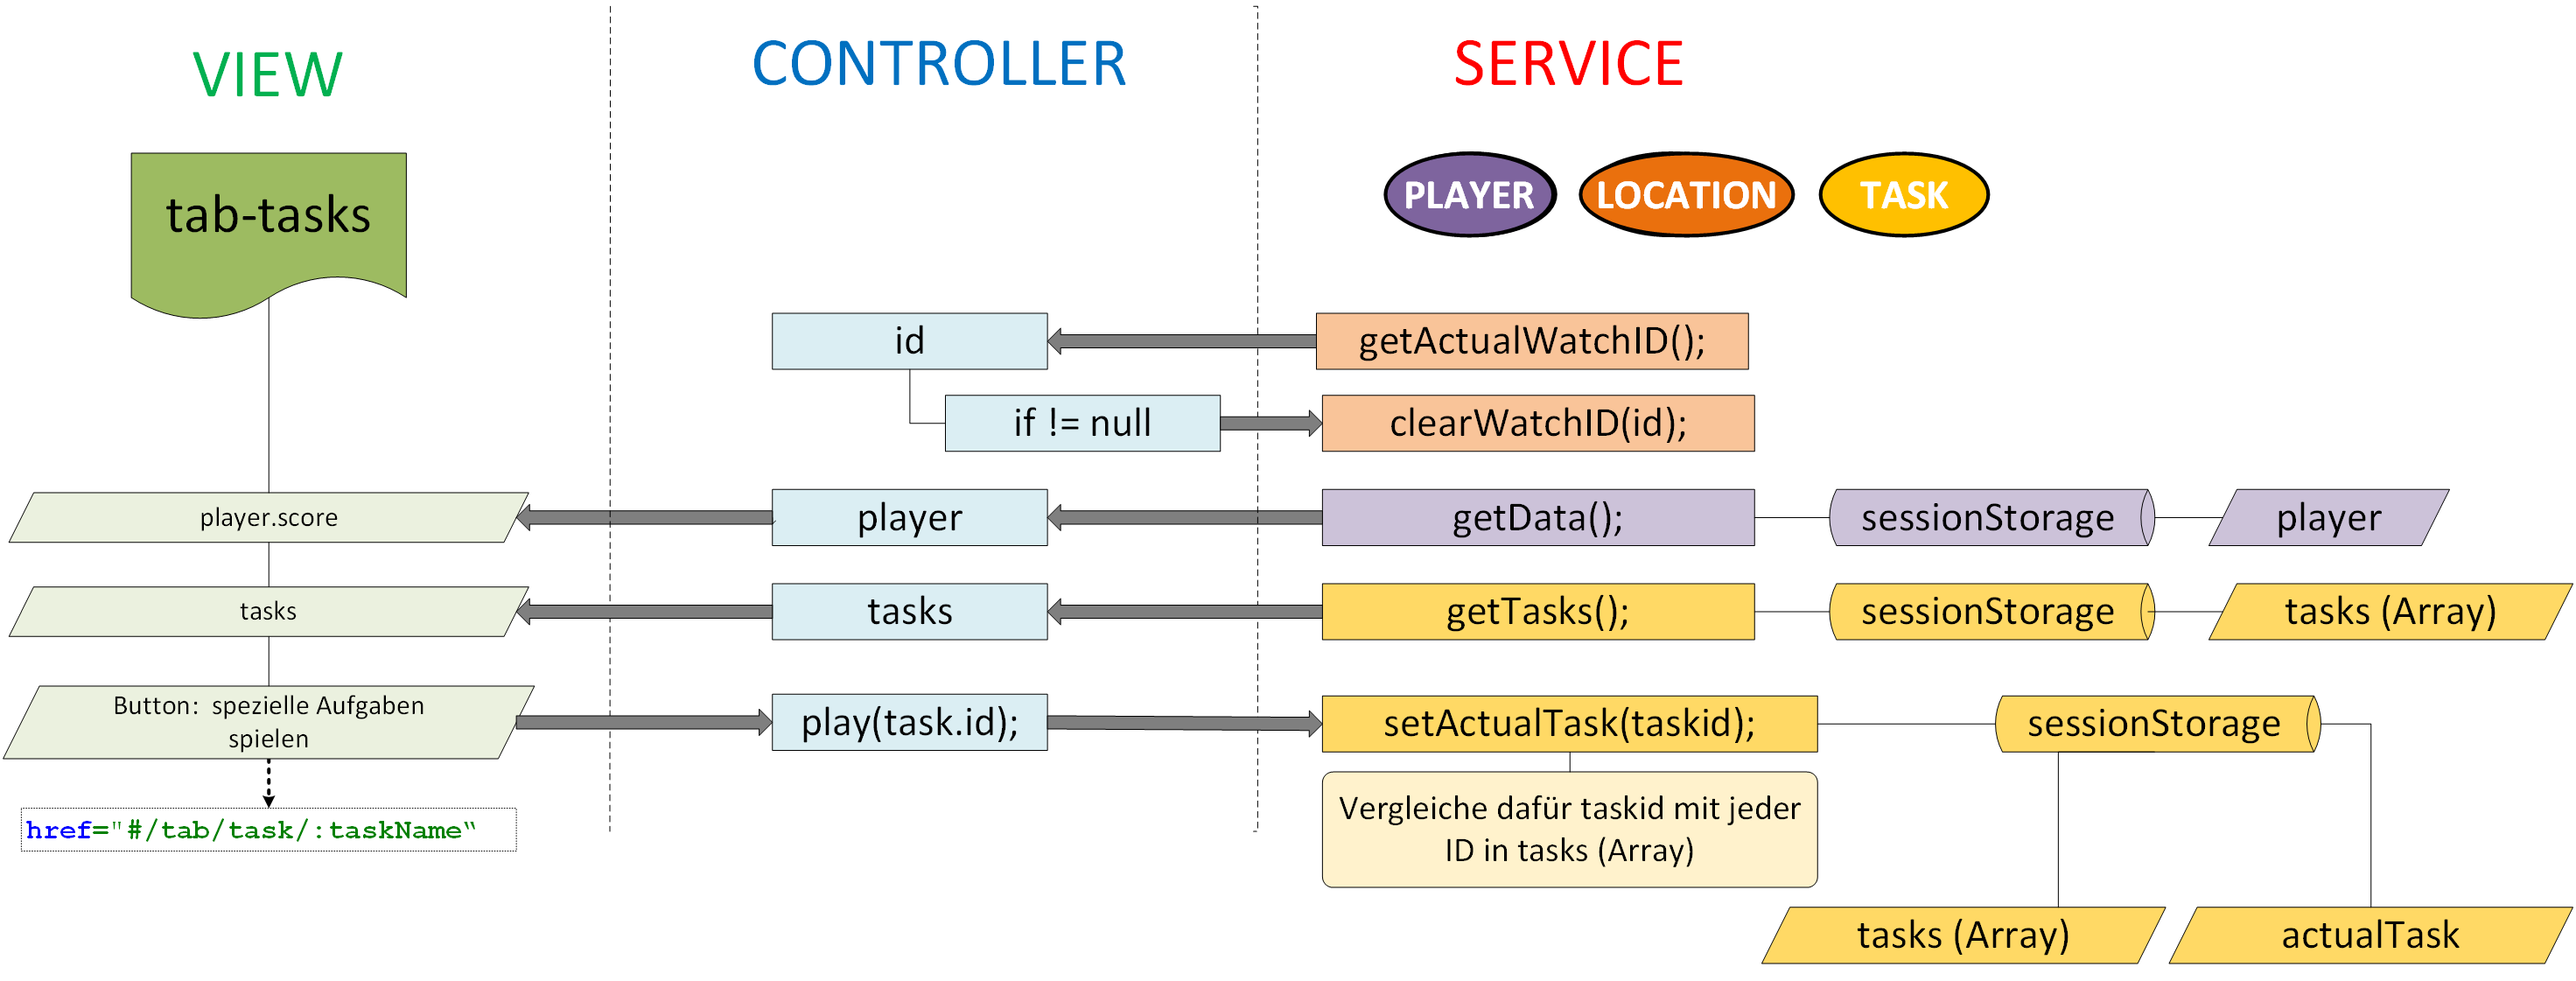
\includegraphics[width=1\textwidth]{ref/images/04-tasks-tab.png}
\caption[Model-View-Controller: Tasks-View]{Model-View-Controller: Tasks-View}
\label{fig:MVC:Tasks-View}
\end{figure}
%
% Beschreibung des Controllers und der Services
%


Der Tasks-View wurde über app.js der Controller 'TasksCtrl' zugewiesen, der wiederum Zugang zum Service 'Player' und 'Task' besitzt. Der 'Player'-Service kapselt alle Funktionen, die mit den Nutzerdaten im Zusammenhang stehen und 'Task' hat die volle Übersicht über die Aufgaben des Spielers.
\\
% Verwendungszweck
\\
Dem Nutzer werden seine aktuell erreichen Punkte angezeigt, die über den \emph{Player Service} vom Controller angefragt werden. Genauso bereitet der Controller die Liste der Aufgaben, die er vom \emph{Task Service} erhält für den Nutzer auf indem er eine Liste von Elementen (Button) anzeigt, die zu der jeweiligen Aufgaben führen sollen. Diese Ermittlungen erfolgen vor dem Laden der View.
\\
Ebenfalls vor dem Anzeigen der HTML-Seite prüft der Controller noch, ob bereits die Position des Geräts geprüft wird. Es könnte ja auch sein, dass der Nutzer die Aufgabe, die er gerade spielt abbricht und auf die Seite mit der übersichtlichen Aufgabenliste zurückkehrt. In diesem Fall wird die sogenannte Watch-ID, die mit der Positionsüberwachung vergeben und im Sessionstorage gespeichert wurde, gelöscht (clearWatchID(id)).
\\
Der Nutzer hat dann nach dem Laden der View die Möglichkeit eine Aufgabe auszuwählen, indem er auf einen der Buttons drückt. Damit stößt er im Controller die Funktion 'play' an, der er (über die Auswahl des Button) die entsprechende Aufgaben-ID übergibt. Der Controller startet diese Aufgabe über den \emph{Task Service}, bzw. seine Funktion 'setActualTask(taskID)' während der Nutzer an die Task-View weitergeleitet wird.
\paragraph{Task-View}
%
%Beschreibung der HTML-Seite
%
Die Task-View ist die Übersichtsseite für eine Aufgabe. Dem Spieler wird die Startentfernung, sein aktueller Punktestand für diese eine Aufgabe genannt. Außerdem bekommt er, wie bei einer Wünschelrute einen Hinweis, ob er sich vom Ziel entfernt oder ob er sich ihm nähert. Dieser Hinweis erscheint nur, wenn er sich auch bewegt, das heißt, wenn sich der Abstand zum Ziel ändert. Ab diesem Moment findet die Positionierung durch die Applikation durchgängig statt.
%
%Ablaufplan
%
\begin{figure}[h]
\centering
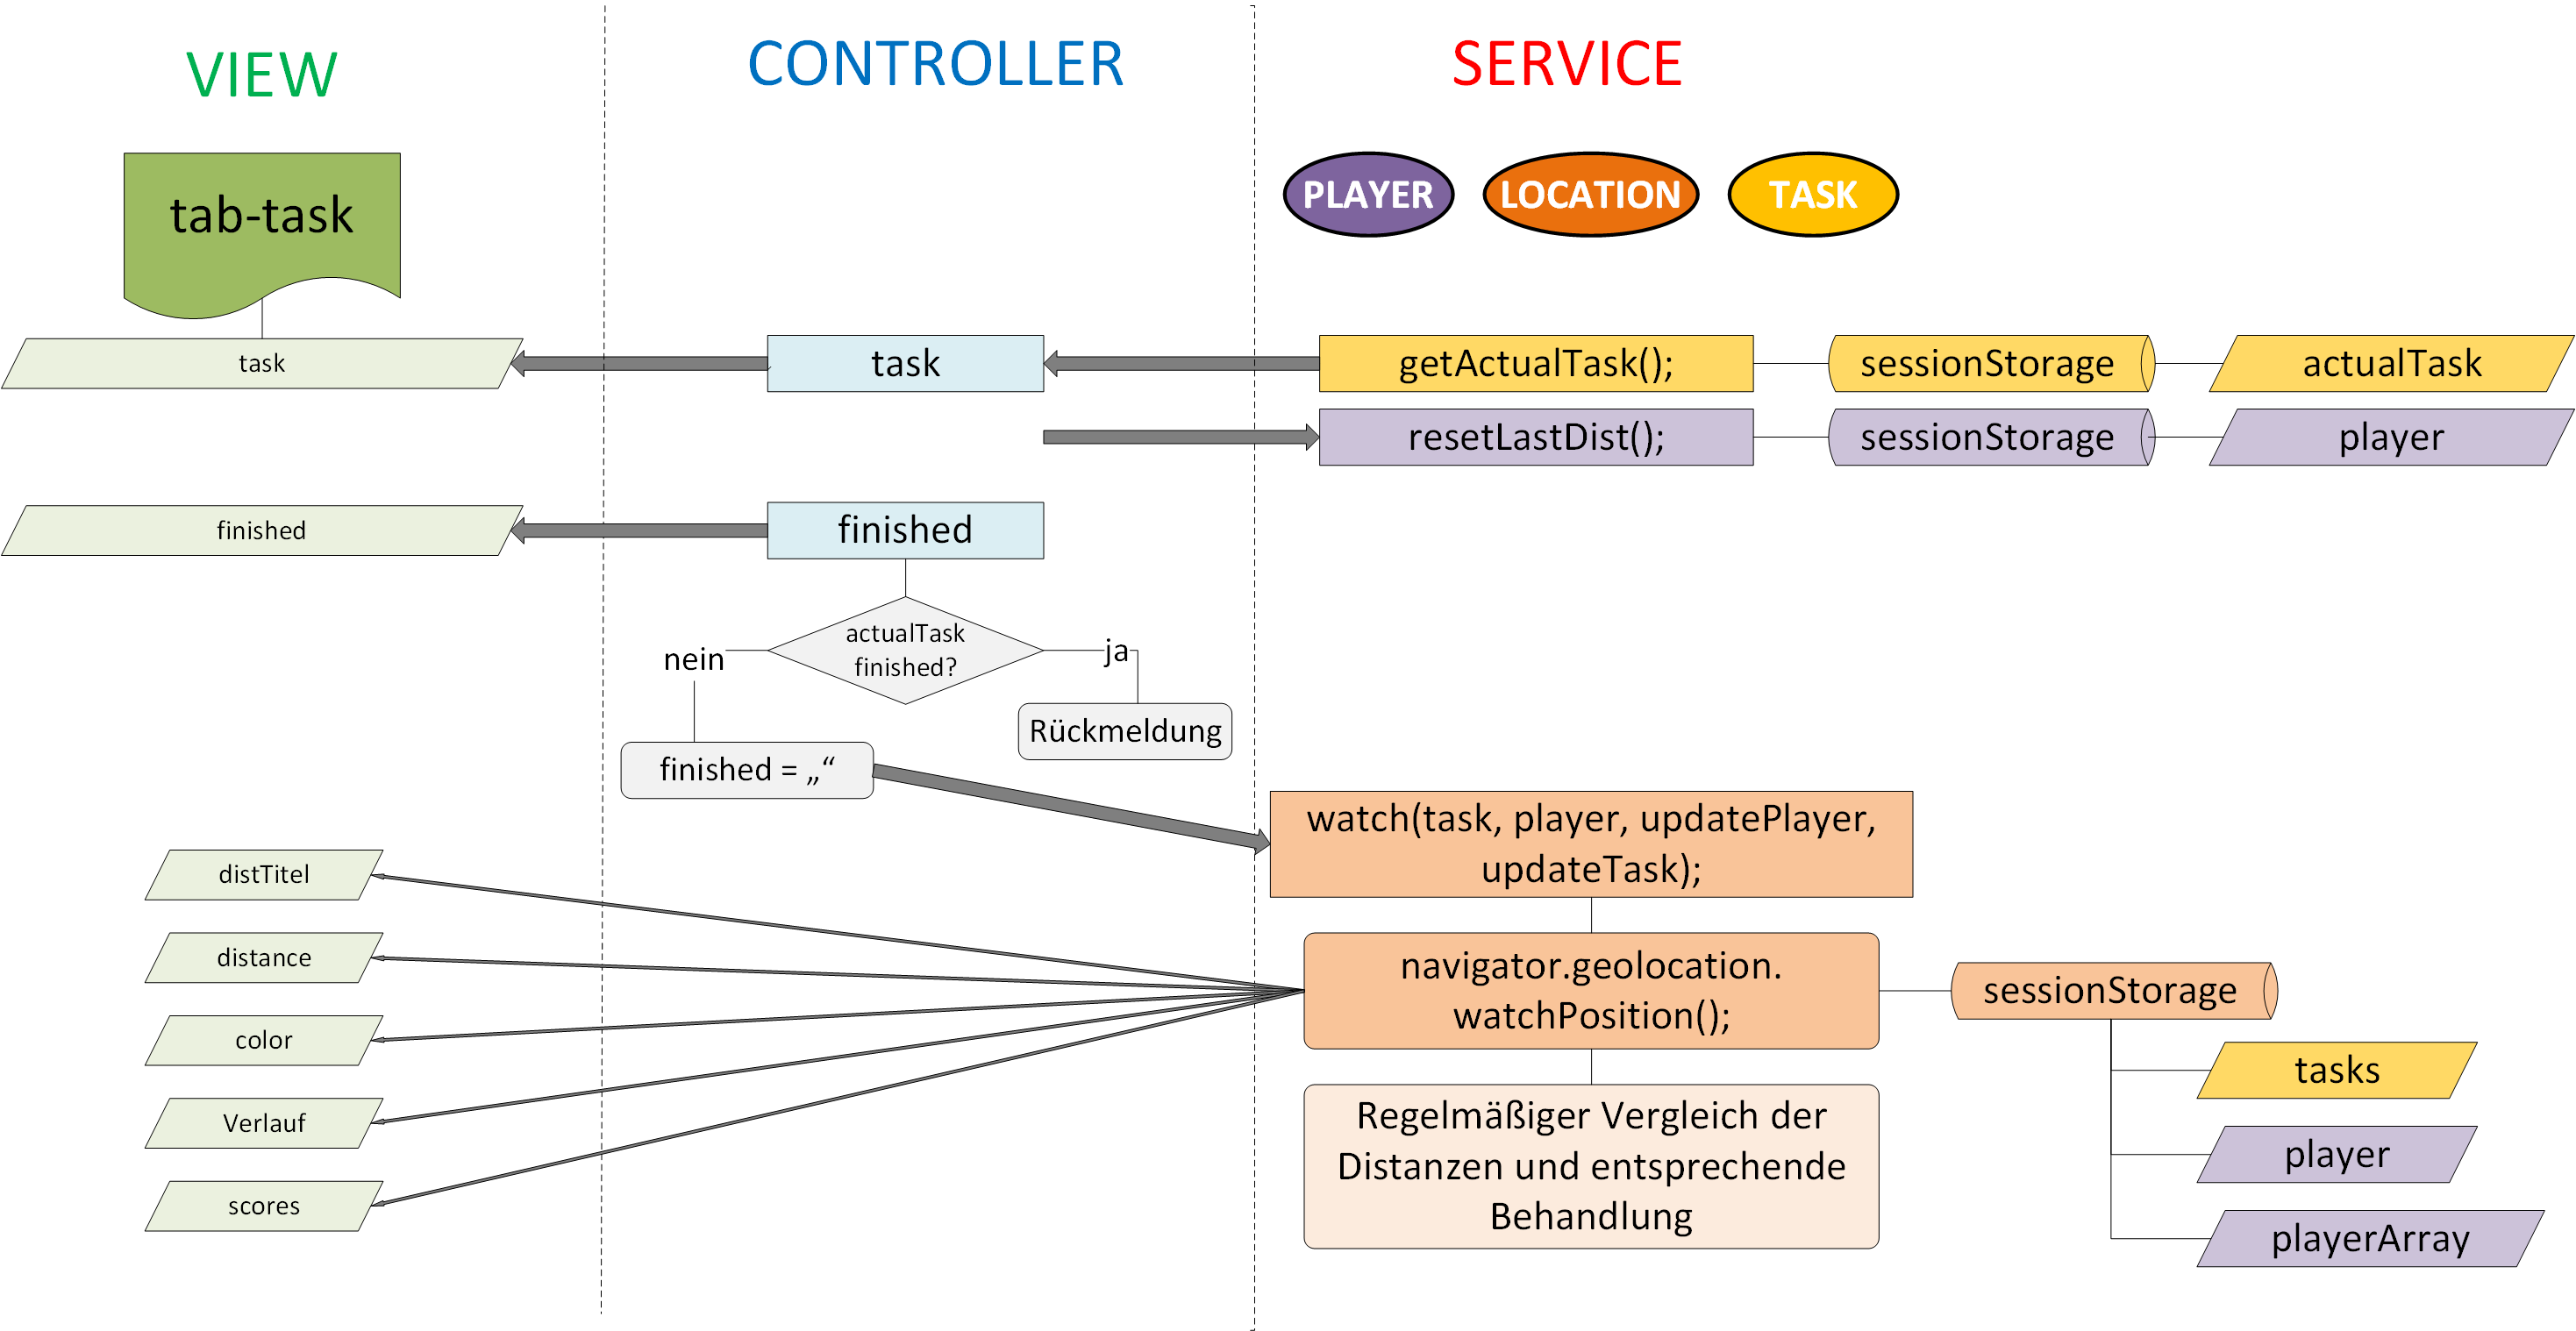
\includegraphics[width=1\textwidth]{ref/images/05-task-tab.png}
\caption[Model-View-Controller: Task-View]{Model-View-Controller: Task-View}
\label{fig:MVC:Task-View}
\end{figure}
%
% Beschreibung des Controllers und der Services
%


Der Task-View wurde über app.js der Controller 'TaskCtrl' zugeordnet. Dieser sorgt dafür, dass die Informationen über die Aufgabe angezeigt werden. Dafür hat er Zugriff auf den \emph{Task Service}, bei dem er über die Task-ID alles über die Aufgabe erfahren kann. Die akutelle Task-ID wurde zuvor vom \emph{Task Service} im Sessionstorage abgelegt und kann jederzeit eingesehen ('getActualTask'-Funktion) und bei Bedarf auch wieder gelöscht werden.
\\
Die Ermittlung der aktuellen Aufgabe und ihrer Informationen findet ebenfalls wieder vor dem Laden der View statt. Genauso muss vor dem Anzeigen auch die letzte gemessene Distanz zurückgesetzt werden. Dafür ist der \emph{Player Service} zuständig, da es sich bei der Distanz um einen spielerbezogenen Wert handelt. Dafür ruft der Controller die Funktion 'resetLastDist' auf, über die der \emph{Player Service} diese Angabe des Spielers auf die Startdistanz der Aufgabe initialisiert.


Wenn der Controller dann feststellt, dass die Aufgabe noch nicht zu Ende gespielt wurde (Prüfung des stateFinished), kann das Spiel beginnen und der \emph{Location Service} startet die Funktion 'watch'. Wenn das Spiel bereits erfolgreich durchlaufen wurde, wird dies dem Nutzer über eine entsprechende Meldung (finished) mitgeteilt, ansonsten bleibt die Variable ohne Textinhalt.


Die 'watch'-Funktion des \emph{Location Service} nutzt wie auch bei der Startpositionsbestimmung den 'navigator.geolocation'. Dieser besitzt eine Funktion 'watchPosition', die eine ID zurückgibt (im Sessionstorage hinterlegt) und solange die Position bei Änderung ermittelt bis die ID gelöscht wird (clearWatch(ID)).
\\
Der Ablauf bei erfolgreicher Positionsbestimmung besagt, dass dem Nutzer jeweils seine neue Distanz, die Tendenz über eine farbliche Daumengeste, sowie die neue Punktzahl entsprechend Annäherung/Entfernung angezeigt werden (distTitel, distance, color, Verlauf, scores). Bei Annäherung bekommt der Spieler einen Punkt dazu bei Entfernung einen Punkt abgezogen.
\\
Wenn die Distanz kleiner als zehn Meter beträgt, gilt die Aufgabe als absolviert. Dafür bekommt der Spieler zehn Punkte und die Watch-ID wird gelöscht. Außerdem werden in diesem Fall die Aufgabe, bzw. der Score für diese Aufgabe und die Gesamtpunkte für den Spieler aktualisiert und gespeichert.


Bei Fehlern bei der Positionsbestimmung erfolgt eine Fehlermeldung nachdem die Timeout-Zeit von 60 Sekunden abgelaufen ist. Die Zeit ist bei der 'watch'-Funktion doppelt so hoch eingestellt, wie bei der Erstbestimmung. Die Erstbestimmung muss für den Nutzer ersichtlich schnell geschehen. Wenn er erst einmal eine Aufgabe verfolgt, kann es schneller mal passieren, dass das Gerät die Position verliert. Sie sollte jedoch sehr robust gegen 'GPS-Löcher' sein und daher wurde die Zeit in dem Fall sehr hoch gewählt, sodass es zu keinem Aufgabenabbruch kommt. In diesem Fall wird natürlich auch die Watch-ID gelöscht.
\subsubsection[Highscores-Tab]{Highscores-Tab
 \\ \textnormal{\small{\textit {Verfasst von Melanie Hammerschmidt}}}}
 
Der Highscores-Tab besteht im Gegensatz zum Spielen-Tab lediglich aus einer View - der Highscores-View.
\begin{figure}[h]
\centering
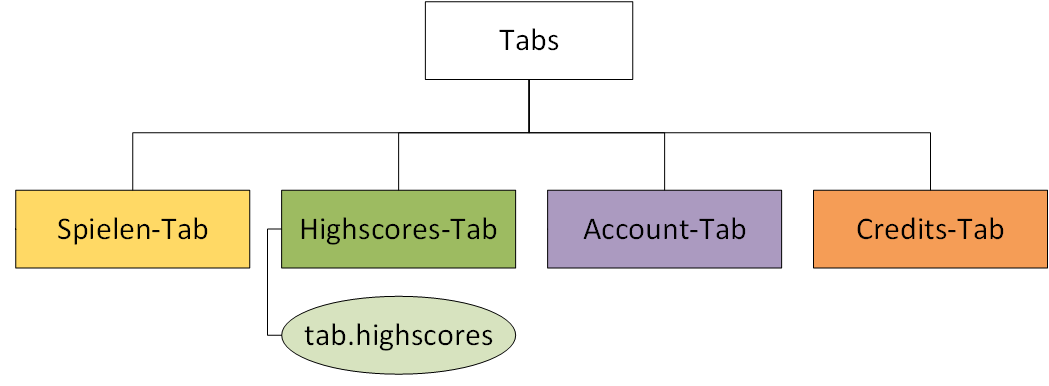
\includegraphics[width=1\textwidth]{ref/images/tabs_highscores.png}
\caption[Tabaufbau Highscores-Tab]{Tabaufbau Highscores-Tab}
\label{fig:Tabaufbau Highscores-Tab}
\end{figure}


\paragraph{Highscores-View}
%
%Beschreibung der HTML-Seite
%
Diese View ist die Übersichtsseite für alle gespeicherten Highscores.
%
%Ablaufplan
\begin{figure}[h]
\centering
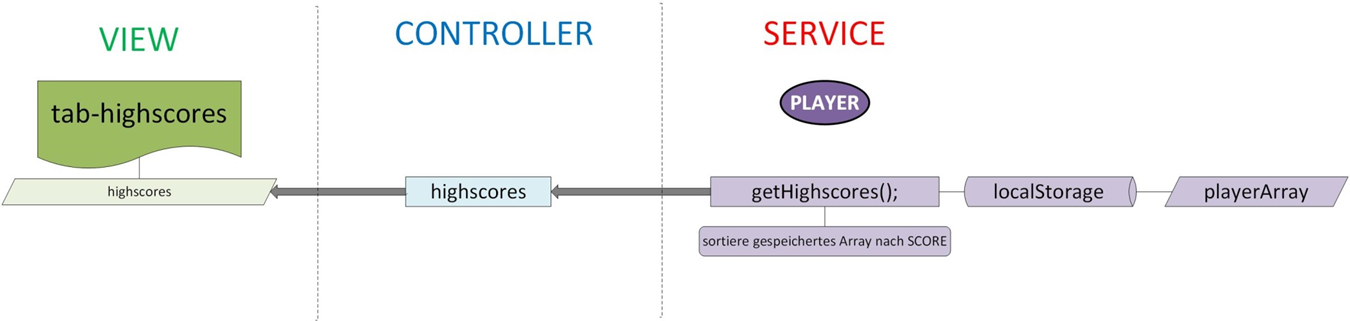
\includegraphics[width=1\textwidth]{ref/images/06-highscores-tab.png}
\caption[Model-View-Controller: Highscores-View]{Model-View-Controller: Highscores-View}
\label{fig:MVC:Highscores-View}
\end{figure}


%
% Beschreibung des Controllers und der Services
Der Highscores-View wurde über app.js der Controller 'HighscoresCtrl' zugewiesen, der Zugriff auf den \emph{Player Service} hat.
\\
Der Controller ist lediglich für die Anzeige von Highscore-Daten zuständig und besitzt daher keine Funktionen, die über die View aufgerufen werden können. Allerdings lädt er vor der Anzeige der View die Highscore-Daten, die der \emph{Player Service} über die Funktion 'getHighscores' anbietet.
\\
Der \emph{Player Service} lädt dafür das Spielerarray, welches im Localstorage des Geräts hinterlegt wurde und sortiert es absteigend. Die Highscore-View zeigt dann lediglich die Spieler des Arrays in dieser Reihenfolge an und gibt die Hintergrundinformationen Spielername, Radius, Zeitpunkt der letzten Änderung und Punktzahl mit an.
\subsubsection[Account-Tab]{Account-Tab
 \\ \textnormal{\small{\textit {Verfasst von Melanie Hammerschmidt}}}}
 
Der Account-Tab besteht ebenfalls aus einer einzigen View - der Account-View.
\begin{figure}[h]
\centering
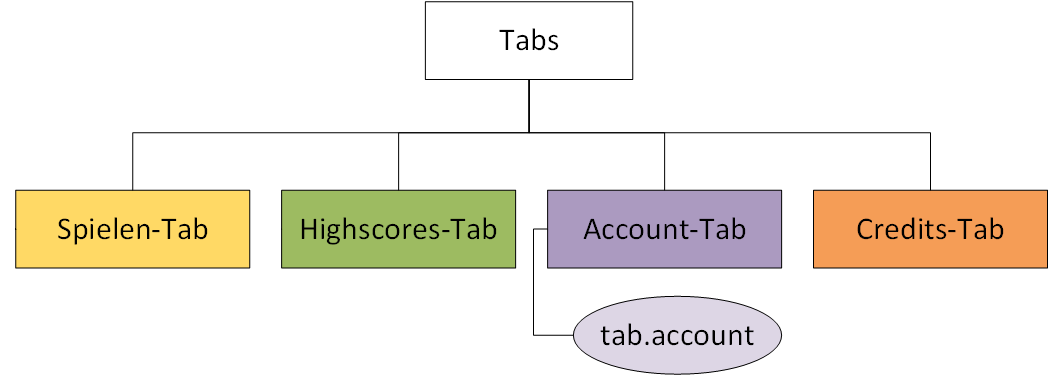
\includegraphics[width=0.7\textwidth]{ref/images/tabs_account.png}
\caption[Tabaufbau Account-Tab]{Tabaufbau Account-Tab}
\label{fig:Tabaufbau Account-Tab}
\end{figure}

\paragraph{Account-View}
%
%Beschreibung der HTML-Seite
%
Die View ist für verschiedene Einstellungen gedacht, die der Spieler der Applikation geben können soll. Im Prototypen wurde an dieser Stelle der Reset-Button zum Zurücksetzen der Highscores implementiert.
%
%Ablaufplan
%
\begin{figure}[h]
\centering
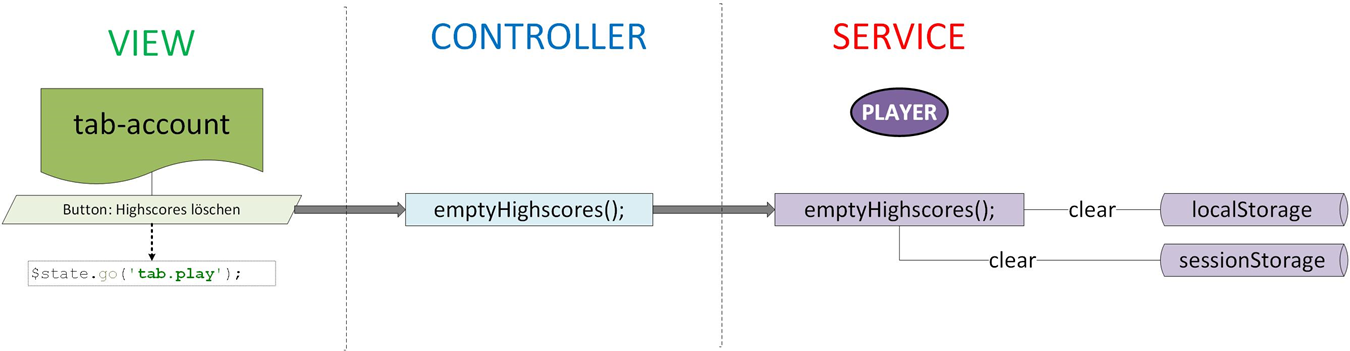
\includegraphics[width=1\textwidth]{ref/images/07-account-tab.png}
\caption[Model-View-Controller: Account-View]{Model-View-Controller: Account-View}
\label{fig:MVC:Account-View}
\end{figure}
%
% Beschreibung des Controllers und der Services
%


Der Account-View wurde über app.js der Controller 'AccountCtrl' zugewiesen, der Zugriff auf den \emph{Player Service} hat.
\\
Mit Klick auf den Button 'Highscores löschen' werden über den Controller bzw. über den \emph{Player Service} alle Daten aus dem lokalen und dem Sessionstorage gelöscht ('emptyHighscores'-Funktion). Im Anschluss daran wird der Nutzer auf die Startseite (Play-View) zurückgeleitet.
\subsubsection[Credits-Tab]{Credits-Tab
 \\ \textnormal{\small{\textit {Verfasst von Melanie Hammerschmidt}}}}
 
Der Credits-Tab besteht ebenfalls aus einer einzigen View - der Credits-View.
\begin{figure}[h]
\centering
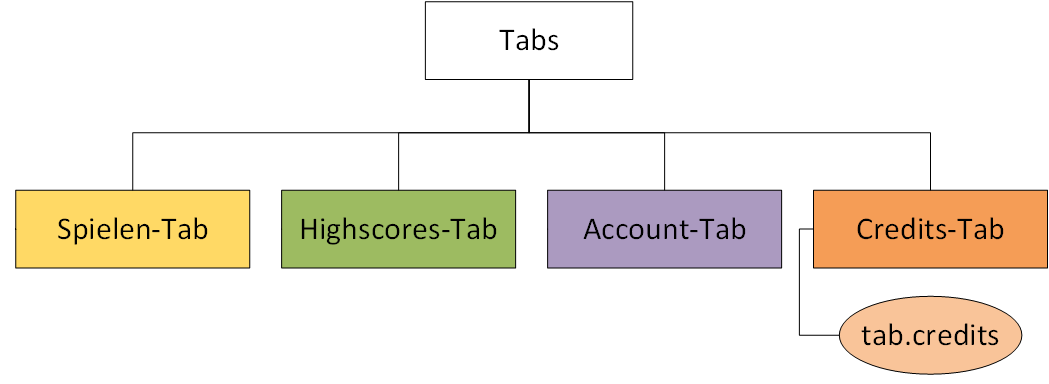
\includegraphics[width=1\textwidth]{ref/images/tabs_credits.png}
\caption[Tabaufbau Credits-Tab]{Tabaufbau Credits-Tab}
\label{fig:Tabaufbau Credits-Tab}
\end{figure}

\paragraph{Credits-View}
%
%Beschreibung der HTML-Seite
%
Diese View ist besonders. Ihr wurde zwar ein Controller ('CreditsCtrl') zugewiesen. Da die Danksagungsseite jedoch keinerlei Funktionalität benötigt und auch keine Daten vor dem Laden erhalten muss, kann man sie als einfache HTML-Seite betrachten, die textuellen Inhalt im Original wiedergibt. Es existiert demnach auch kein Ablaufplan.
\newpage
\subsubsection[Übersicht]{Übersicht
 \\ \textnormal{\small{\textit {Verfasst von Melanie Hammerschmidt}}}}
 
Die drei Services \emph{Player}, \emph{Location} und \emph{Task} werden je nach Aufgabenstellung von den Controllern benötigt. Jeder Funktionsaufruf eines Service brauch dafür zuerst eine feste Verbindung vom Controller zu dem Service. Die Abhängigkeitsstruktur der Applikation sieht so aus:
\begin{figure}[h]
\centering
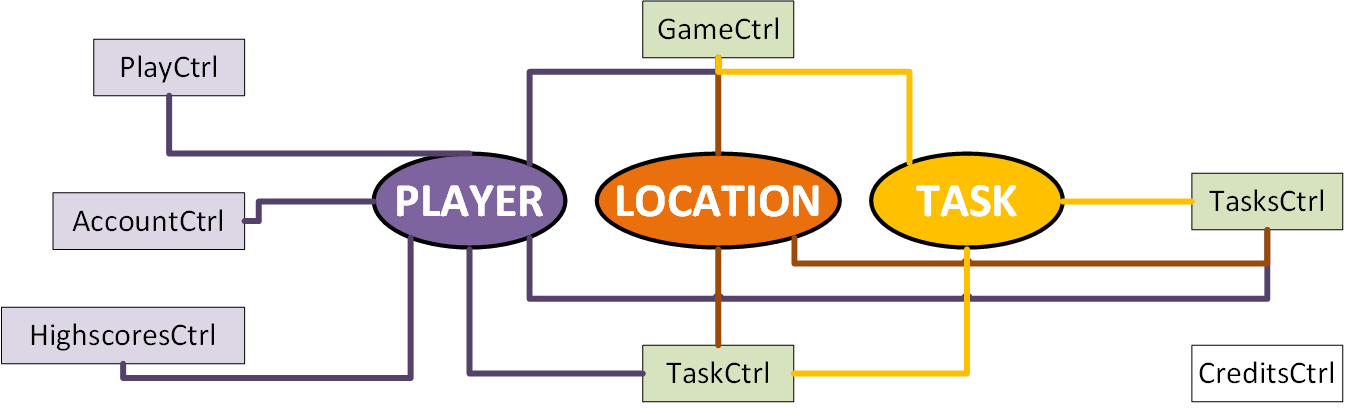
\includegraphics[width=1\textwidth]{ref/images/controller_services.png}
\caption[Übersicht Controller-Services Verbindungen]{Übersicht Controller-Services Verbindungen}
\label{fig:Controller-Services}
\end{figure} 

Wie in den vorherigen Abschnitten beschrieben existiert ein reger Informationsaustausch zwischen den Views, den Controllern und Services. Dieser ist symptomatisch für die Model-View-Controller-Architektur, wie bereits in Kapitel \ref{sec:Architektur} beschrieben und sorgt für größtmögliche Unabhängigkeit zwischen den Elementen, da lediglich die Schnittstellen(Funktionsparameter) von Bedeutung sind und somit auch große Wiederverwertbarkeit gegeben ist.
\\
Von der Applikation werden für die in den vorherigen Kapiteln vorgestellten Funktionen verschiedene Plugins genutzt.
Standardmäßig ist das Plugin für Console, Keyboard und Device für Zugriff auf die Grundfunktionen des genutzten Geräts installiert. Für die LBS-spezifischen Funktionen wurde noch das Plugin Geolocation und für die Informationen über die Internetverbindung das Plugin Network Information hinzugefügt. Jedes Plugin muss dafür in der Form '"cordova plugin add ...'" über die Konsole Cordova bekannt gegeben werden.
\subsubsection[Bewertung der Architektur]{Bewertung der Architektur
 \\ \textnormal{\small{\textit {Verfasst von Melanie Hammerschmidt}}}}
Nach der Implementierung ist der Rückbezug auf die anfangs gemachten Anforderungen relevant.
\\
Die fachlichen Anforderungen wurden großteils erfüllt. Pro Spieler wird in Speicher des Geräts ein Objekt gespeichert, das die Grundeinstellungen (Name, Spielradius, Startposition) hält. Diese Anforderungen werden vom Player Service übernommen.
\\
Auch die Aufgabenerstellung wird anhand der Startposition und des Radius ermittelt. Das war ebenfalls eine fachliche Aufgabenstellung und wird in der Architektur vom Task Service übernommen. Der Ansatz des steigenden Schwierigkeitsgrads wurde im Prototypen nicht weiter verfolgt, ebenso wie das Verfolgen der Höhe des Spielers.
\\
Die Höhe war technisch betrachtet zu schwer festzulegen. Die Angaben der Testgeräte waren zu ungenau, um daraus ein wiederholbares, einfaches Konzept zu implementieren. Der steigende Schwierigkeitsgrad könnte durch ein weiteres Detail in der Aufgabendefinition (Schwierigkeitsgrad) implementiert werden und die Aufgaben daher bei der Ermittlung über die jeweilige Entfernung in beispielsweise drei Kategorien eingeteilt werden. Dementsprechend könnten dann auch mehr Punkte bei Erreichen des Ziels verrechnet werden.
Dies ist nur ein Beispiel für Erweiterungen des Prototypen bevor er zu einer produktiven Applikation würde.
\\
Bei der Aufgabendurchführung wurden alle Anforderungen erfüllt. Die Aufgaben werden beim Spielen ständig verfolgt und der Prototyp gibt ständig Rückmeldung. Außerdem ist die Möglichkeit, das Spiel zu pausieren sowie die Tatsache einer immer aktuelle Highscoreberechnung gegeben.
\\
\\
Die Bewertung der technischen, nicht-funktionalen Anforderungen fällt ebenfalls sehr positiv aus. Die Plattformunabhängigkeit ist durch die Umstände der hybriden Architektur gegeben.
\\
Um die tatsächliche Benutzbarkeit des Prototypen zu testen wäre eine umfassende Usability-Prüfung nötig. Die Auffassung der Entwickler und einzelner Tester der Umgebung ist jedoch, dass die Applikation übersichtlich zu steuern war. Dies ist gegeben durch den getabbten Aufbau der Anwendung. 
\\
Die Selbstbeschreibungsfähigkeit ist dadurch gewährleistet, dass bei der Entwicklung darauf geachtet wurde, dem Nutzer ständig Rückmeldung zu geben. Außerdem ist die Architektur möglichst einfach gehalten, was ebenfalls zu einer erleichterten Bedienung beiträgt.
\\
Durch vergleichbare Applikationen ist auch die Erwartungskonformität hoch, da bei der Entwicklung auch vergleichbare Applikationen im Vorfeld hinzugezogen wurden.
\\
Die Fehlertoleranz einer Applikation, die auf Location Based Services aufbaut muss unbedingt hoch sein. Bei fehlerhafter Lokalisierung muss die Applikation unbedingt eine entsprechende Fehlerroutine durchlaufen. Dies ist im Prototypen gegeben, der jeden technischen Fehler abfängt und dem Nutzer der Anwendung schriftlich aufbereitet. Außerdem muss in solch einem Fall die Lokalisierung beendet werden, da man sonst in eine Endlosschleife geraten könnte.
\\
Die Animation des '"Wünschelrouteneffekts'" ist im Prototypen noch relativ einfach implementiert. Es wird dem Nutzer lediglich die Entfernung in entsprechender Farbe (rot für weiter weg und grün für näher dran) dargestellt. Eine Optimierung der Animation einer zu verkaufender Applikation wäre noch wünschenswert, für einen Prototypen, der die technischen Fähigkeiten einer Location Based Services Applikation werden daher aber auch schon schön veranschaulicht.
\\
Abschliessend lässt sich sagen, dass der Aufbau der Applikation, wie in der Architektur beschrieben sehr strukturiert durchgezogen wurde, was vor allem an dem speziellen Angular JS Aufbau mittels Views, Controller und Services liegt. Das einfache Austauschen einzelner Komponenten hat die Entwicklung des Rahmenwerks vereinfacht, was den kreativen Teil der Implementierung gestärkt hat. Auch die gelungene Betriebssystemunabhängigkeit passt sich in das allgemein positive Resumee ein.
\subsection[Umsetzung iBeacons]{Umsetzung iBeacons
 \\ \textnormal{\small{\textit {Verfasst von Victor Schwartz}}}}

Unter der Voraussetzung, dass die definierten Zielpunkte der App mit jeweils einem iBeacon ausgestattet werden. Können diese, die Genauigkeit der Entfernung verbessern.
Hierfür muss die App Signale des iBeacons empfangen. Deshalb läuft während der gesamten Ortungsphase im Hintergrund ein iBeacon Scanner. Sobald dieser Scanner den gewünschten iBeacon entdeckt hat wird die Distanz zum Ziel durch den iBeacon bestimmt und nicht per GPS, dadurch wird eine höhere Genauigkeit im Zielgebiet erreicht.

Um dies zu implementieren, muss das Zielpunkt Objekt angepasst werden. Standortobjekte benötigen neben Namen und Positionen noch eine iBeacon ID sowie Major und Minor Werte.

Mit den neuen Werten sind alle Vorraussetzungen geschaffen um einen iBeacon Scanner zu implementieren. Hierfür wird das Plug-In "Cordova / Phonegap iBeacon plugin" von Peter Metz verwendet. \cite{petermetz} Es ist open Source und kann von Git Hub heruntergeladen werden.

Das Plug-In enthält Schnittstellen und Funktionen zum finden von iBeacons. Hierbei werden zwei unterschiedliche Funktionalitäten geboten.


1. Monitoring von iBeacons
\\Beim Monitoring wird ständig überprüft ob das Smartphone welches das Plug-In nutzt in einen Bereich eintritt, indem ein iBeacon Signale sendet. Ebenfalls wird überprüft ob das Smartphone den Bereich verlässt. Diese Funktion wird in dieser Arbeit genutzt um dem User anzuzeigen, dass bei Eintritt in eine iBeacon Zone nicht mehr GPS genutzt wird, sondern die Abstandsbestimmung mit Hilfe des iBeacons erfolgt.

2. Ranging von iBeacons
\\Während Monitoring nur den Aus- bzw. Einritt in eine Zone überprüft, ermittelt das iBeacon Ranging alle in der nähe befindlichen iBeacons und gibt eine ungefähre Distanz zu diesen an. Diese Funktionalität wird genutzt um die Distanz zum Zielort in der App darzustellen.\cite{MonitorRange}


Im folgenden wird die Umsetzung anhand von Quellcode Beispielen erläutert:

Installation
\\Damit das Plug-In genutzt werden kann, muss es erst über die Console des Betreibssystem installiert werden.
Hierfür navigiert man in der Console zum Hauptordner der App. Dort führt man den Befehl:

\begin{lstlisting}
cordova plugin add com.unarin.cordova.beacon
\end{lstlisting} 


aus. Draufhin erfolgt die automatische Installation im Ordner "plugin" der App und es kann auf die Schnittstellen zugegriffen werden.

Der allgemeine Ablauf besteht aus mehreren Schritten:
\begin{enumerate}
\item Schritt Anlegen eines Obejkt mit iBeacon Informationen
\item Schritt Hauptfunktion aufrufen
\item Schritt Warten auf einen iBeacon in Reichweite
\item Schritt Daten auslesen
\end{enumerate}
Diese Schritte werden im folgenden mit Quellcode-Listings aus der App erläutert:

1. Anlegen eines Objekt mit iBeacon Information
\\Wie bereits in Kapitel \ref{sec:ibeacons} erläutert, senden Beacons mehrere Informationen in einem definierten Zeitabstand. Hierzu zählt die UUID, eine eindeutige Zahlen und Buchstabenkombination sowie eine Major und Minor Nummer. Mit Hilfe dieser Daten lässt sich ein Beacon identifizieren. Da jedes Ziel mit einem iBeacon ausgestatte werden soll, muss die App hierfür jeweils diese Daten kennen. Aus diesem Grund gibt es ein Objekt mit diesen Daten.
 
\begin{lstlisting}[frame=single]  % Start your code-block

var mRegions =
				[
					{
						id: 'region1',
						uuid: '95F428B1-4A3A-4E39-B086-21BFF38DEB6D',
						major: 0,
						minor: 304
					}
				];
\end{lstlisting}


2. Hauptfunktion aufrufen
\\Damit nach dem iBeacon durch die App gesucht wird, muss 'Ranging' und 'Monitoring' gestartet werden. Dieses überwacht ob sich der iBeacon in Reichweite befindet. Hierfür wird die Funktion 'startMonitoringAndRangingRegion' aufgerufen. Beim Aufruf dieser Funktion wird das Objekt mit den iBeacon Daten 'mRegions' mit übergeben. Mit diesen Daten wird ein neues Objekt vom Typ BeaconRegion erstellt. Dieses Obejekt wird von den Funktionen  cordova.plugins.locationManager.startRangingBeaconsInRegion(beaconRegion) und cordova.plugins.locationManager.startMonitoringForRegion(beaconRegion) verwendet um das Ranging und Monitoring nach diesem iBeacon zu starten.

\begin{lstlisting}[frame=single]  % Start your code-block

function startMonitoringAndRangingRegion(region, errorCallback)
				{
					// Create a region object.
					
					var beaconRegion = new cordova.plugins.locationManager.BeaconRegion(
						region.id,
						region.uuid,
						region.major,
						region.minor);

					// Start ranging.
					cordova.plugins.locationManager.startRangingBeaconsInRegion(beaconRegion)
						.fail(errorCallback)
						.done();

					// Start monitoring.
					cordova.plugins.locationManager.startMonitoringForRegion(beaconRegion)
						.fail(errorCallback)
						.done();
				}
\end{lstlisting}


3. Warten auf iBeacon in Reichweite
\\Die im vorherigen Schritt beschriebene Funktion lässt die App im Hintergrund nach dem iBeacon suchen. Befindet sich der gesuchte iBeacon in Reichweite und das Bluetooth Modul des Smartphones empfängt Signale wird folgende Funktion aufgerufen:

\begin{lstlisting}[frame=single]  % Start your code-block

function onDidRangeBeaconsInRegion(result)
					{
						globalBeacons = result.beacons;
					}
\end{lstlisting}

Diese Funktion enthält die empfangenen Informationen des iBeacons in der Variable 'result'. Damit die Informationen global verwendet werden können, werden diese in die Variable 'globalBeacons' geschrieben. Der Vorteil ist, im Gesamten Dokument kann nun auf diese Informationen zugegriffen werden. Somit ist es möglich eine Fallunterscheidung zu treffen ob die Entfernung für das Spiel per GPS/Wlan bestimmt oder über einen iBeacon ermittelt werden kann.


4. Daten auslesen
\\Nachdem die Daten des iBeacons im Objekt globalBeacons abgespeichert wurden kann auf die übermittelte Distanz wie folgt zugegriffen werden:

\begin{lstlisting}[frame=single]  % Start your code-block

					dist = globalBeacons.accuracy;
					
\end{lstlisting}


Mit diesen Funktionen und Daten kann eine Fallunterscheidung erfolgen ob die Distanz per GPS/Wlan oder mit den Daten des iBeacon bereit gestellt wird.
Mit einer zusätzlichen Variable 'beaconfound' wird die Fallunterscheidung vereinfacht. Diese Variable ist entweder 'false' oder 'true', je nachdem ob der gesuchte iBeacon in Reichweite ist oder nicht. Die beiden folgenden Screenshots zeigen auf, welche Unterscheidungen und Veränderungen in der App angezeigt werden, wenn GPS/Wlan oder iBeacons verwendet werden.

\begin{figure}
\centering
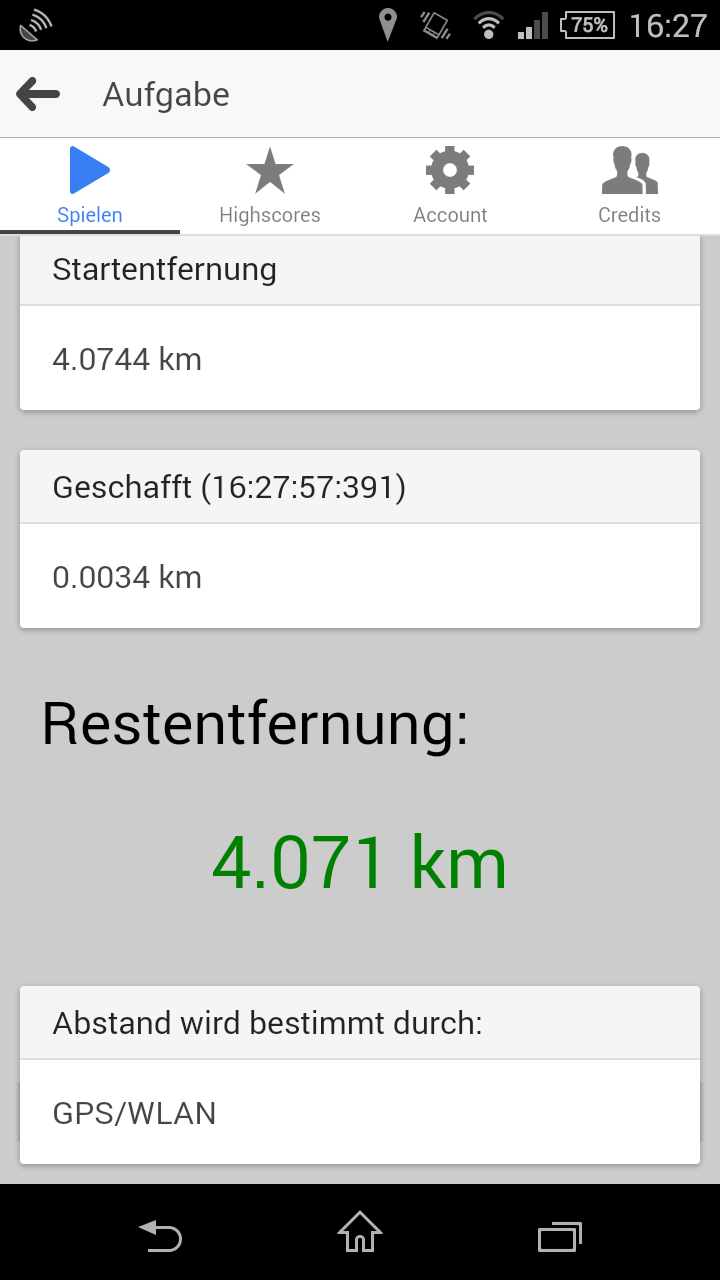
\includegraphics[width=0.3\textwidth]{ref/images/screenshot1.png}
\caption[Screenshot des Prototypen mit GPS-Ortung]{Screenshot des Prototypen mit GPS-Ortung}
\label{fig:screenshotapp1}
\end{figure} 

\begin{figure}
\centering
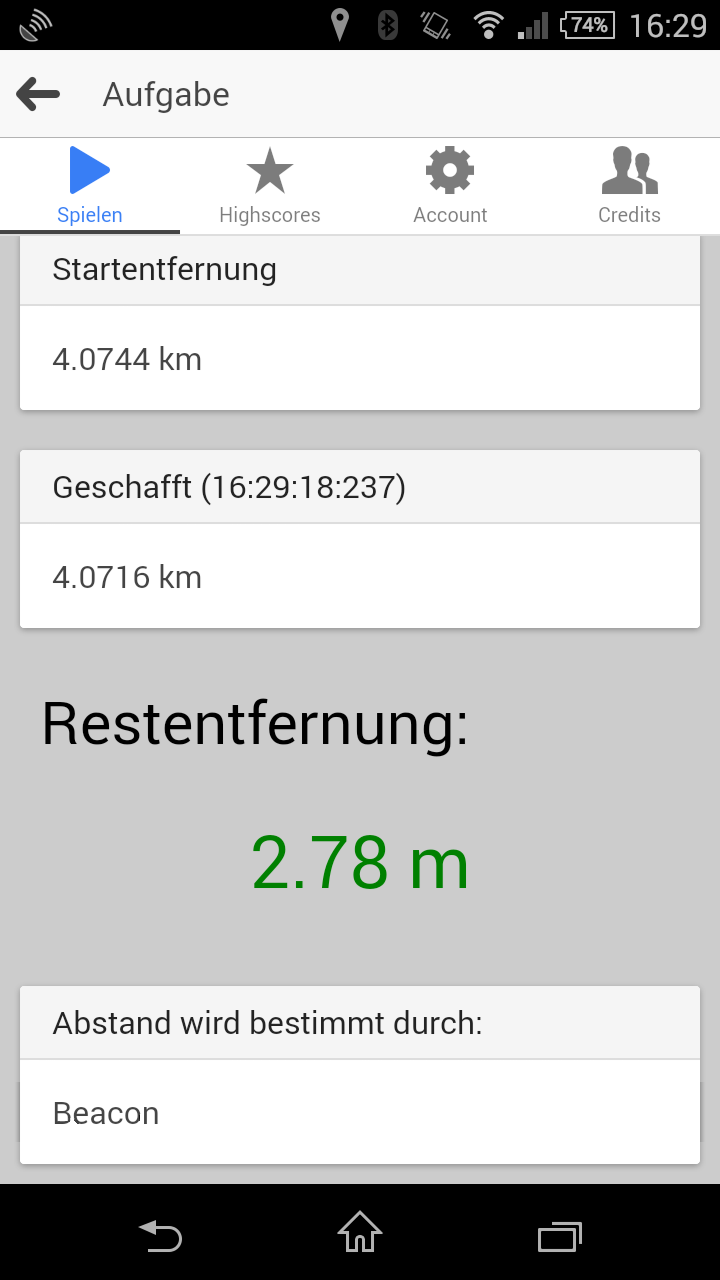
\includegraphics[width=0.3\textwidth]{ref/images/screenshot2.png}
\caption[Screenshot des Prototypen mit iBeacon Nutzung]{Screenshot des Prototypen mit iBeacon Nutzung}
\label{fig:screenshotapp2}
\end{figure} 
%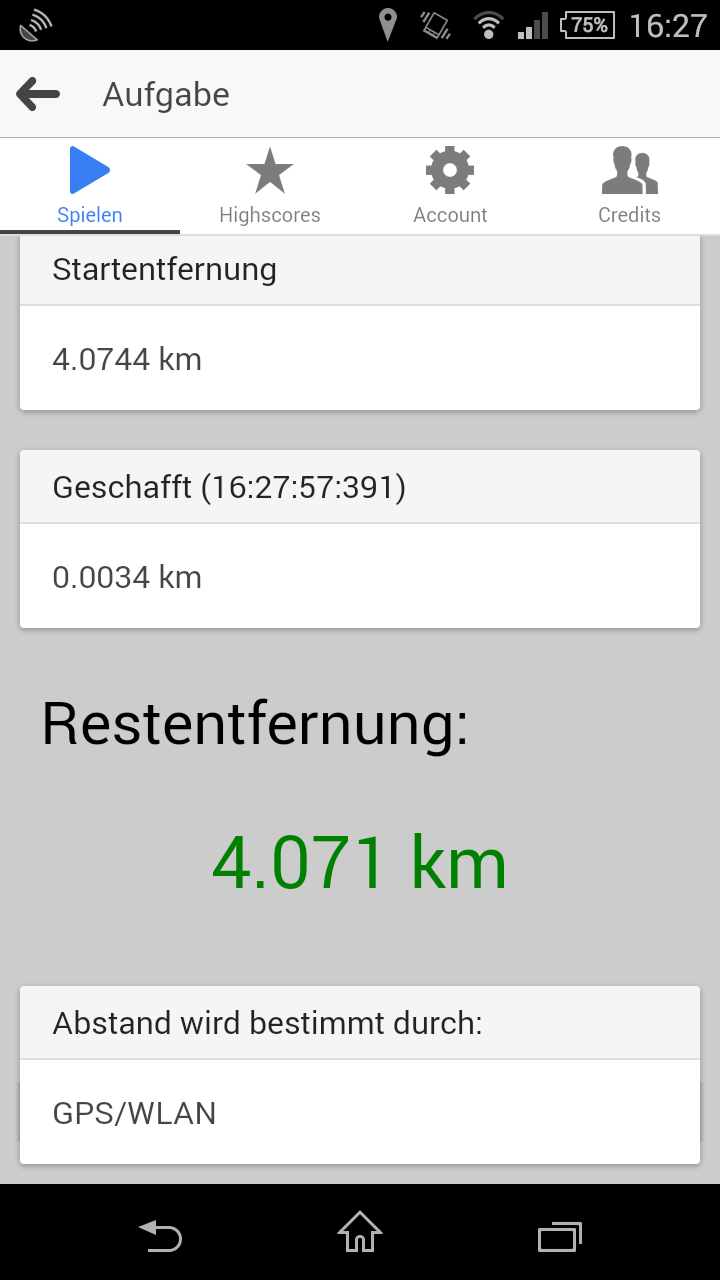
\includegraphics[width=0.3\textwidth]{ref/images/screenshot1.png} 
%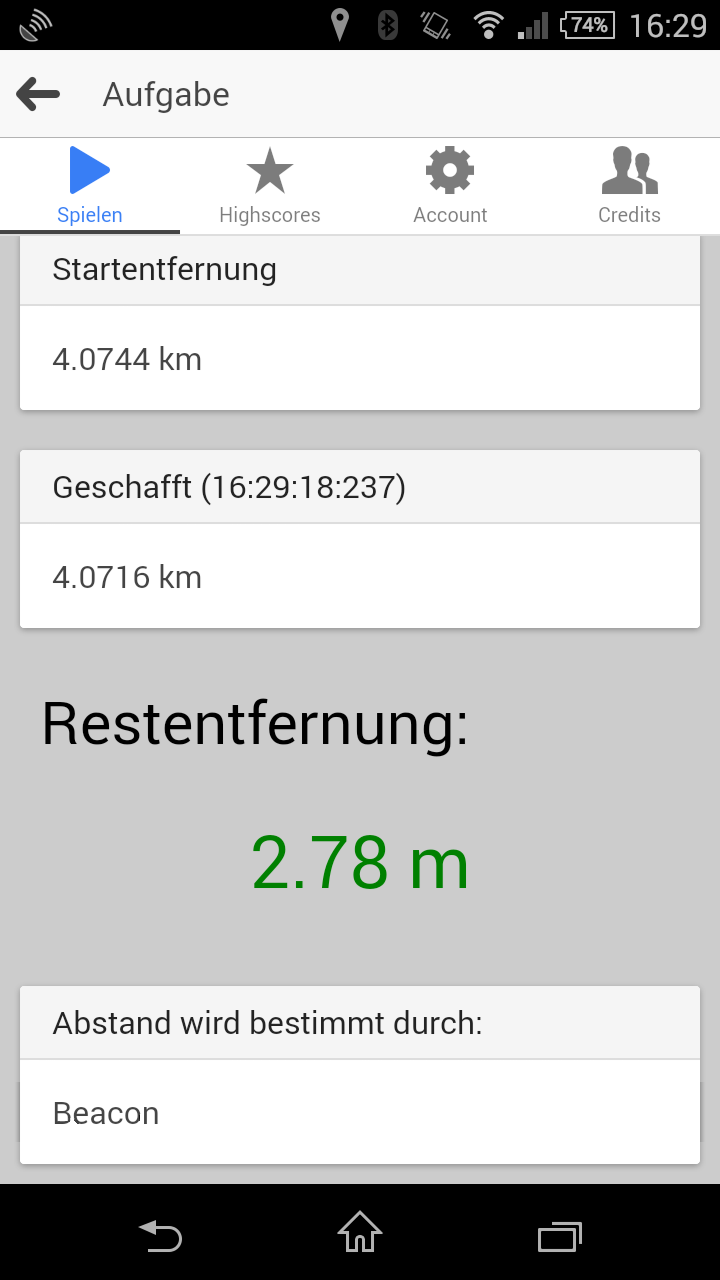
\includegraphics[width=0.3\textwidth]{ref/images/screenshot2.png} 
Auf beiden Bilder (\ref{fig:screenshotapp1} und \ref{fig:screenshotapp2}) ist die App abgebildet. Sie zeigt jeweils an wie weit das Ziel noch entfernt ist. Im linken Bild wird die Entfernung mit Hilfe von GPS bestimmt. Im rechten Bild findet die Bestimmung der Entfernung per Beacon statt.
Per Fallunterscheidung wird das Anzeigefeld angepasst. Damit weiß der Nutzer, mit welchem System der Abstand bestimmt wird. Des Weiteren wird die Entfernung nicht in km angegeben sondern in Metern, da die Enfernungsbestimmtung mit einem iBeacon wesentlich genauer ist als mit GPS.

